
\subsection{Amplificadores con operacionales}

\label{section:modelo_operacional}

En esta sección analizamos distintas configuraciones con amplificadores operacionales, pero teniendo en cuenta ciertos aspectos de los amplificadores operacionales reales, en particular usamos un modelo lineal, y lo analizamos a bajas/medias frecuencias, sin tener en cuenta en principio el ancho de banda, ni cosas como el \textit{slew rate}, que corresponden a efectos que no se pueden modelar linealmente. El modelo utilizado es el mostrado en la figura~\figref{fig:fig_operational_non_ideal}, como se puede ver, solo consideramos, una ganancia de tensión diferencial de valor finito, una resistencia de entrada también finita y una resistencia de salida mayor a $0$.

\begin{figure}[H] %htb
\begin{center}
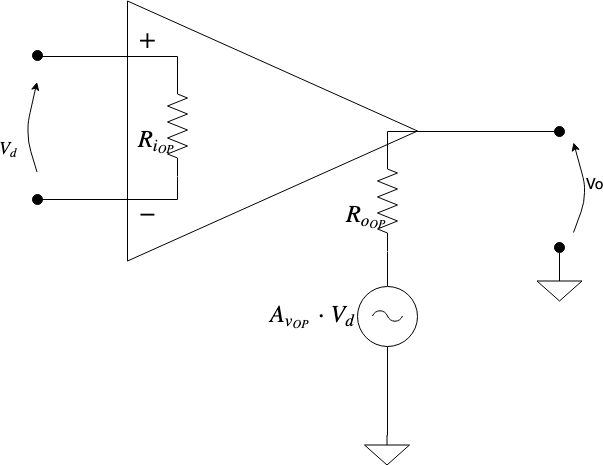
\includegraphics[width=1 \textwidth, angle=0]{./img/operacionales/OP_NONIDEAL_MODEL.png}
\caption{\label{fig:fig_operational_non_ideal}\footnotesize{Modelo lineal de un operacional no ideal.}}
\end{center}
\end{figure}

\vfill

\clearpage

\subsubsection{Amplificador no inversor}

Usando el modelo descripto en la sección~\sectref{section:modelo_operacional} analizamos el circuito mostrado en la figura~\figref{fig:fig_operational_ideal_non_inverter}. El circuito es un amplificador no inversor con amplificador no operacional. El análisis que se hará por realimentación, pretende analizar como es la transferencia de mismo con nuestro modelo, y como influye la no idealidad del operacional en la transferencia, para finalmente ver a que se reduce la transferencia al llevar las expresiones al caso ideal.

\begin{figure}[H] %htb
\begin{center}
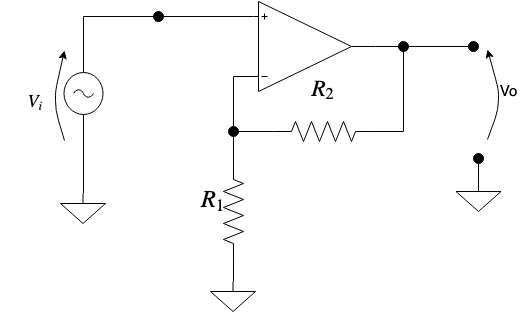
\includegraphics[width=0.5 \textwidth, angle=0]{./img/operacionales/OP_NINV.png}
\caption{\label{fig:fig_operational_ideal_non_inverter}\footnotesize{Amplificador no inversor.}}
\end{center}
\end{figure}




\subsubsection{Amplificador inversor}


\subsubsection{Amplificador diferencial}